		Rewriting \eqref{eq:chapters/11/11/5/6/parabola} in matrix form,
    \begin{align}
        \vec{x}^\top\myvec{1&0\\0&0}\vec{x} + 2\myvec{0&-6}\vec{x} = 0
        \label{eq:chapters/11/11/5/6/parabola-mtx}
    \end{align}
    The above parabola can be  expressed in standard form using 
\begin{align}
	\vec{x} = \vec{P}\vec{y} = \myvec{0 & 1 \\ 1 & 0}\vec{y}
        \label{eq:chapters/11/11/5/6/affine}
\end{align}
yielding
    \begin{align}
        \vec{y}^\top\myvec{0&0\\0&1}\vec{x} + 2\myvec{-6&0}\vec{x} = 0
        \label{eq:chapters/11/11/5/6/parabola-mty}
    \end{align}
    Hence, 
    from
\eqref{eq:conic_quad_form_nc}, 
    \begin{align}
	    \vec{n} = \vec{e}_1
        \label{eq:chapters/11/11/5/6/n}
	\\
	    c = -\frac{36}{2\times 6} = -3
    \end{align}
    Substituting in 
  \eqref{eq:conic_quad_form_F} 
  yields
    \begin{align}
        \vec{F} = 3\vec{e}_1
    \end{align}
    Thus, the equation of the latus rectum is
\begin{align}
        \vec{x} = \vec{F} + \kappa \vec{e}_2
        \label{eq:chapters/11/11/5/6/x-general}
    \end{align}
        Substituting in \eqref{eq:chapters/11/11/5/6/parabola-mty} and simplifying,
    \begin{align}
\kappa = \pm 6
        \label{eq:chapters/11/11/5/6/x-latus}
    \end{align}
    Thus, the ends of the latus rectum are
    \begin{align}
        \vec{y} = \myvec{3 \\ \pm 6}
    \end{align}
    The relevant parameters with respect to 
        \eqref{eq:chapters/11/11/5/6/parabola-mtx}
	can now be obtained using 
        \eqref{eq:chapters/11/11/5/6/affine}.
See \figref{fig:chapters/11/11/5/6/parabola}.
The area of the required triangle is
    \begin{align}
        \textrm{ar}\brak{\triangle OAB} = \frac{1}{2}\mydet{6&3\\-6&3} = 18 
    \end{align}
    \begin{figure}[H]
        \centering
        %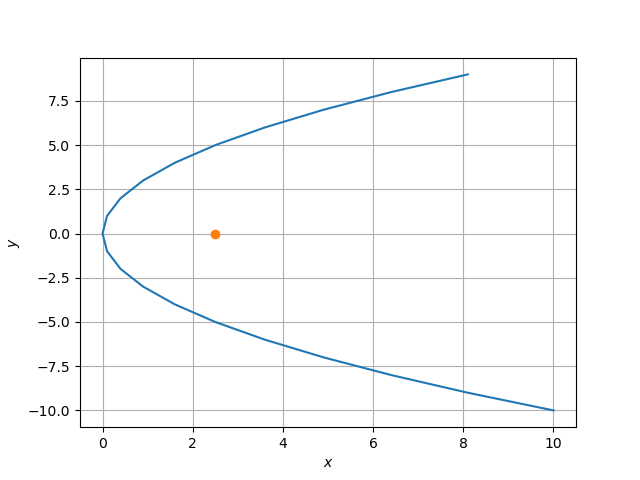
\includegraphics[width=0.75\columnwidth]{chapters/11/11/5/6/figs/parabola.png}
        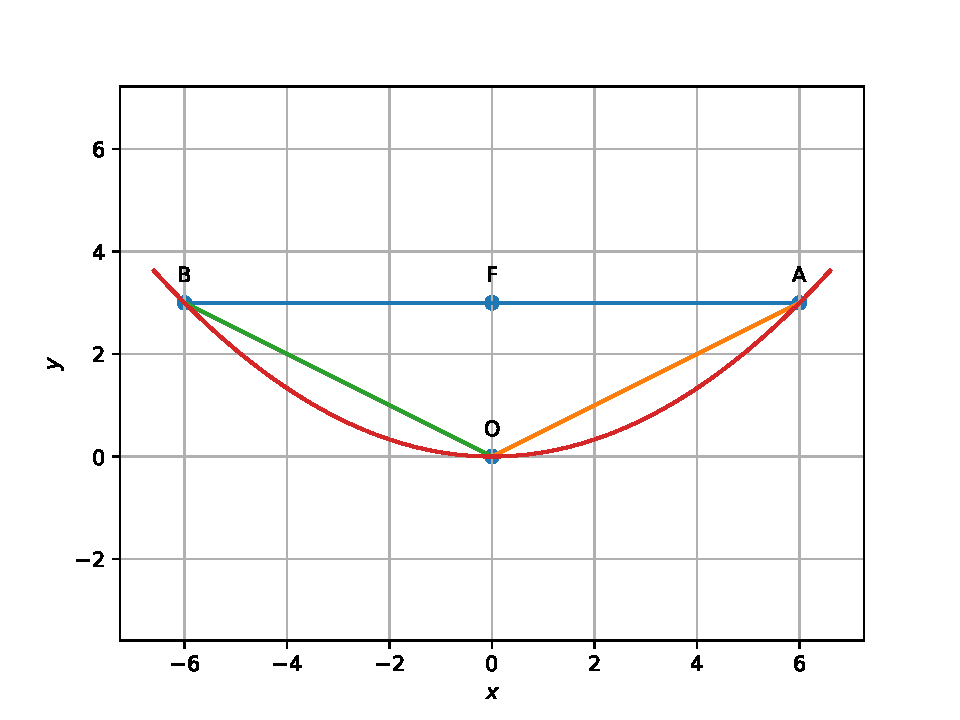
\includegraphics[width=0.75\columnwidth]{chapters/11/11/5/6/figs/fig1.pdf}
        \caption{}
        \label{fig:chapters/11/11/5/6/parabola}
    \end{figure}
